\documentclass[a4paper,10pt]{report}\input{../0.Préambule/Préambule_cours_prof}\begin{document}

\definecolor{titlecolor}{rgb}{0.81, 0.09, 0.13}
\newpage
\setcounter{chapter}{17}
\chapter{Probabilités}

\section{Expériences aléatoire}

\begin{ex}
\begin{enumerate}
\item On lance \href{https://fr.piliapp.com/random/coin/}{une pièce de monnaie} et on regarde la face supérieure.
\item On lance \href{https://fr.piliapp.com/random/dice/}{un dé à six faces} et on regarde le nombre de points inscrits sur la face du dessus.
\item On fait tourner \href{https://fr.piliapp.com/random/wheel/}{une roue marquée} sur ses secteurs de couleurs différentes et on regarde le secteur marqué.
\end{enumerate}
\end{ex}

\begin{dft}
Une expérience (lancé un dé par exemple) est aléatoire lorsqu'elle a plusieurs résultats (pile ou face) et \textbf{que l'on ne peut pas prévoir, à priori, quel résultat se produira .}

\medskip
\noindent Les résultats possibles d'une expérience s'appelle des issues.
\end{dft}

\begin{ex}
On s'intéresse aux situations décrites dans l'\textbf{Exemple 1}.

\medskip \noindent\grandscarreaux{\linewidth}{3.2cm}
\end{ex}

\section{Vocabulaire}

\begin{dft}
Un évènement est constitué par plusieurs issues d'une même expérience aléatoire .
\end{dft}

\begin{ex}
Lors du lancer d'un \href{https://fr.piliapp.com/random/dice/}{dé équilibré à six faces}, on étudie l'événement « obtenir un nombre pair ».

\medskip
\noindent Cet événement est réalisé par les issues : $2$ ; $4$ et $6$.
\end{ex}

\begin{rmq}
Un événement élémentaire est un événement réalisé par une seule issue.
\end{rmq}

\begin{ex}
Toujours lors du lancer du dé décrit ci-dessus, citons un événement élémentaire ...

\medskip \noindent\grandscarreaux{\linewidth}{1.6cm}
... et un événement qui n'est pas élémentaire.

\medskip \noindent\grandscarreaux{\linewidth}{1.6cm}
\end{ex}

\begin{dft}
L'événement contraire d'un événement $A$, noté $\overline{A}$, est celui qui se réalise lorsque l'événement $A$ n'a pas lieu.
\end{dft}

\begin{ex} Lors du lancer du dé précédemment décrit, on considère l'événement $A$ : \og Obtenir un multiple de 3 \fg{}

\medskip
\noindent Il est réalisé \dotfill

\medskip
\noindent L'événement contraire à $A$, noté $\overline{A}$ est \dotfill

\medskip
\noindent Il est réalisé \dotfill
\end{ex}

\section{Notion de probabilité}

\begin{dft}
Lorsque l'on effectue un très grand nombre de fois une expérience aléatoire (de façon indépendante et dans les mêmes conditions), la fréquence de réalisation d'un événement, se rapproche d'un nombre que l'on appelle probabilité de cet événement.
\end{dft}

\begin{ex}
Soit $A$ l'événement \href{https://fr.piliapp.com/random/coin/}{\og j'obtiens pile au lancer d'une pièce de monnaie \fg{}}.

\medskip
\noindent La probabilité pour que $A$ se réalise est \dotfill

\medskip
\noindent On note : \dotfill
\end{ex}

\begin{prop}
La probabilité d'un évènement est un nombre compris entre $0$ et $1$ qui exprime « la chance qu'a un évènement de se produire ».
\end{prop}

\begin{ex}
Dire que la probabilité d'un évènement est de $0,8$ signifie que cet évènement a $8$ chances sur $10$ ou $80 \%$ de chance de se produire.
\end{ex}

\begin{rmq}
\begin{enumerate}
\item[•] Un événement est impossible lorsqu'il ne peut pas se produire. Sa probabilité est égale à $0$.
\item[•] Un événement est certain lorsqu'il se réalise toujours. La probabilité d'un événement certain est égale à $1$.
\end{enumerate}
\end{rmq}

\begin{prop}
La somme des probabilités de tous les événements élémentaires est égale à 1.
\end{prop}

\section{Représentation des événements} 

\noindent \begin{minipage}{8.5cm}
\noindent \textbf{Arbres des possibles}

On lance une pièce de monnaie trois fois de suite, on peut schématiser cette expérience par un arbre :

\begin{center}
% Racine à Gauche, développement vers la droite
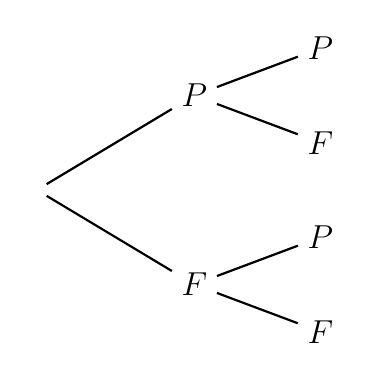
\begin{tikzpicture}[xscale=1,yscale=1,scale=0.6]
% Styles (MODIFIABLES)
\tikzstyle{fleche}=[-,>=latex,thick]
\tikzstyle{noeud}=[fill=white]
\tikzstyle{feuille}=[fill=white]
\tikzstyle{etiquette}=[midway,above]
\tikzstyle{etiquette1}=[midway,below]
% Dimensions (MODIFIABLES)
\def\DistanceInterNiveaux{2}
\def\DistanceInterFeuilles{1}
% Dimensions calculées (NON MODIFIABLES)
\def\NiveauA{(0)*\DistanceInterNiveaux}
\def\NiveauB{(1.6666666666666665)*\DistanceInterNiveaux}
\def\NiveauC{(3)*\DistanceInterNiveaux}
\def\NiveauD{(4)*\DistanceInterNiveaux}
\def\InterFeuilles{(-1)*\DistanceInterFeuilles}
% Noeuds (MODIFIABLES : Styles et Coefficients d'InterFeuilles)
\node[noeud] (R) at ({\NiveauA},{(3.5)*\InterFeuilles}) {};
\node[noeud] (Ra) at ({\NiveauB},{(1.5)*\InterFeuilles}) {\large{$P$}};
\node[noeud] (Raa) at ({\NiveauC},{(0.5)*\InterFeuilles}) {\large{$P$}};
%\node[feuille] (Raaa) at ({\NiveauD},{(0)*\InterFeuilles}) {\large{$P$}};
%\node[feuille] (Raab) at ({\NiveauD},{(1)*\InterFeuilles}) {\large{$F$}};
\node[noeud] (Rab) at ({\NiveauC},{(2.5)*\InterFeuilles}) {\large{$F$}};
%\node[feuille] (Raba) at ({\NiveauD},{(2)*\InterFeuilles}) {\large{$P$}};
%\node[feuille] (Rabb) at ({\NiveauD},{(3)*\InterFeuilles}) {\large{$F$}};
\node[noeud] (Rb) at ({\NiveauB},{(5.5)*\InterFeuilles}) {\large{$F$}};
\node[noeud] (Rba) at ({\NiveauC},{(4.5)*\InterFeuilles}) {\large{$P$}};
%\node[feuille] (Rbaa) at ({\NiveauD},{(4)*\InterFeuilles}) {\large{$P$}};
%\node[feuille] (Rbab) at ({\NiveauD},{(5)*\InterFeuilles}) {\large{$F$}};
\node[noeud] (Rbb) at ({\NiveauC},{(6.5)*\InterFeuilles}) {\large{$F$}};
%\node[feuille] (Rbba) at ({\NiveauD},{(6)*\InterFeuilles}) {\large{$P$}};
%\node[feuille] (Rbbb) at ({\NiveauD},{(7)*\InterFeuilles}) {\large{$F$}};
% Arcs (MODIFIABLES : Styles)
\draw[fleche] (R)--(Ra);
\draw[fleche] (Ra)--(Raa);
%\draw[fleche] (Raa)--(Raaa);
%\draw[fleche] (Raa)--(Raab);
\draw[fleche] (Ra)--(Rab);
%\draw[fleche] (Rab)--(Raba);
%\draw[fleche] (Rab)--(Rabb);
\draw[fleche] (R)--(Rb);
\draw[fleche] (Rb)--(Rba);
%\draw[fleche] (Rba)--(Rbaa);
%\draw[fleche] (Rba)--(Rbab);
\draw[fleche] (Rb)--(Rbb);
%\draw[fleche] (Rbb)--(Rbba);
%\draw[fleche] (Rbb)--(Rbbb);
\end{tikzpicture}
\end{center}
\end{minipage}
\hspace{5mm}
\begin{minipage}{7.5cm}
\textbf{Tableaux à doubles entrées}

On jette deux dés à quatre faces (tétraèdre régulier) et on regarde le résultat obtenu :

\begin{center}
\renewcommand{\arraystretch}{1.65}
\begin{tabular}{|*{5}{C{0.7}|}}
\hline 
\rowcolor{lightgray!50}& \textbf{1} & \textbf{2} & \textbf{3} & \textbf{4} \\\hline
\cellcolor{lightgray!50}{\textbf{1}} & $\left\lbrace 1; 1 \right\rbrace$ & $\left\lbrace 2 ; 1 \right\rbrace$ & $\left\lbrace 3 ; 1 \right\rbrace$ & $\left\lbrace 4 ; 1 \right\rbrace$ \\\hline
\cellcolor{lightgray!50}{\textbf{2}} & $\left\lbrace 1; 2 \right\rbrace$ & $\left\lbrace 2 ; 2 \right\rbrace$ & $\left\lbrace 2 ; 3 \right\rbrace$ & $\left\lbrace 2 ; 4 \right\rbrace$ \\\hline 
\cellcolor{lightgray!50}{\textbf{3}} & $\left\lbrace 3 ; 1 \right\rbrace$ & $\left\lbrace 3 ; 2 \right\rbrace$ & $\left\lbrace 3 ; 3 \right\rbrace$ & $\left\lbrace 3 ; 4 \right\rbrace$ \\\hline 
\cellcolor{lightgray!50}{\textbf{4}} & $\left\lbrace 4 ; 1 \right\rbrace$ & $\left\lbrace 4 ; 2 \right\rbrace$ & $\left\lbrace 4 ; 3 \right\rbrace$ & $\left\lbrace 4 ; 4 \right\rbrace$ \\\hline 
\end{tabular} 
\end{center}
\end{minipage}

\end{document}